\chapter{高级I/O编程}
\label{chp:Advanced-IO-programming}

\section*{基本信息}
\sline
\begin{description}
\item[课程名称:] Java应用与开发
\item[授课教师:] 王晓东
\item[授课时间:] 第七周
\item[参考教材:] 本课程参考教材及资料如下:
  \begin{itemize}
  \item 陈国君主编,Java程序设计基础(第5版),清华大学出版社,2015.5
  \item Bruce Eckel, Thinking in Java (3rd)
  \end{itemize}
\end{description}

\section*{教学目标}

\sline

\begin{enumerate}
\item 深入理解Java的I/O原理
\item 掌握Java基本I/O流类型
\item 掌握I/O的几种应用编程方式
\end{enumerate}

\section*{授课方式}

\sline
\begin{description}
\item[理论课:] 多媒体教学、程序演示
\item[实验课:] 上机编程
\end{description}

\newpage
\section*{教学内容}
\sline

%%%%%%%%%%%%%%%%%%%%%%%%%%%%%%%%%%%%%%%%%%%%%%%%%%%%%%%%%%%%%%
\section{Java I/O原理}

\subsection{Java I/O原理}

\subsubsection{ I/O(Input/Output)基本概念}

\begin{itemize}
\item 数据源(Data Source)
\item 数据宿(Data Sink)
\item 流(Stream)\\
  {\kai Java中把不同的数据源与程序间的数据传输都抽象表述为流,java.io包中定义
    了多种I/O流类型实现数据I/O功能。}
\end{itemize}

\subsection{Java I/O流的分类}

\subsubsection{按照数据流动的方向}

{\hei Java流可分为输入流(Input Stream)和输出流(Output Stream)。}

\begin{itemize}
\item 输入流只能从中读取数据,而不能向其写出数据;
\item 输出流则只能向其写出数据,而不能从中读取数据。
\item {\Mage (特例 java.io.RandomAccessFile类)}
\end{itemize}


\subsubsection{根据数据流所关联的是数据源还是其他数据流}  

{\hei 可分为节点流(Node Stream)和处理流(Processing Stream)。}

\begin{itemize}
\item 节点流直接连接到数据源;
\item 处理流是对一个已存在的流的连接和封装,通过所封装的流的功能调用
  实现增强的数据读/写功能,处理流并不直接连到数据源。
\end{itemize}

\begin{figure}[htb]
  \centering
  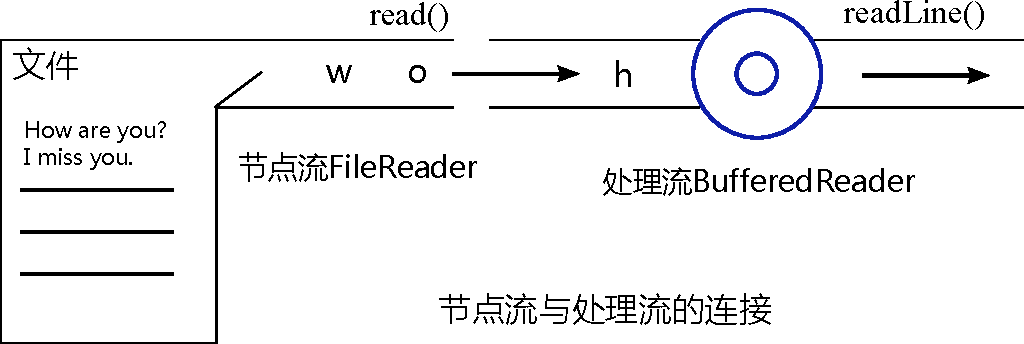
\includegraphics[width=0.8\textwidth]{images/Advanced-IO-programming/fig-stream-link.pdf}
  \caption{InputStream和OutputStream}
  \label{fig:fig-stream-link}
\end{figure}

\subsubsection{按传输数据的“颗粒大小”}

{\hei 可分为字符流(Character Stream)和字节流(Byte Stream)。}

\begin{itemize}
\item 字节流以字节为单位传输数据,每次传送一个或多个字节。
\item 字符流以字符为单位传输数据,每次传送一个或多个字
  符。\footnote{从JDK1.4版本开始,Sun公司引入了新的Java I/O
    API(NIO, New Input/Output),提供面向数据块、异步I/O操作。}
\end{itemize}

\notice{Java命名惯例}

凡是以InputStream或OutputStream结尾的类型均为{\hei 字节流},凡是
以Reader或Writer结尾的均为{\hei 字符流。}

\section{基础I/O流}

\subsection{InputStream and OutputStream}

\begin{figure}[htb]
\centering
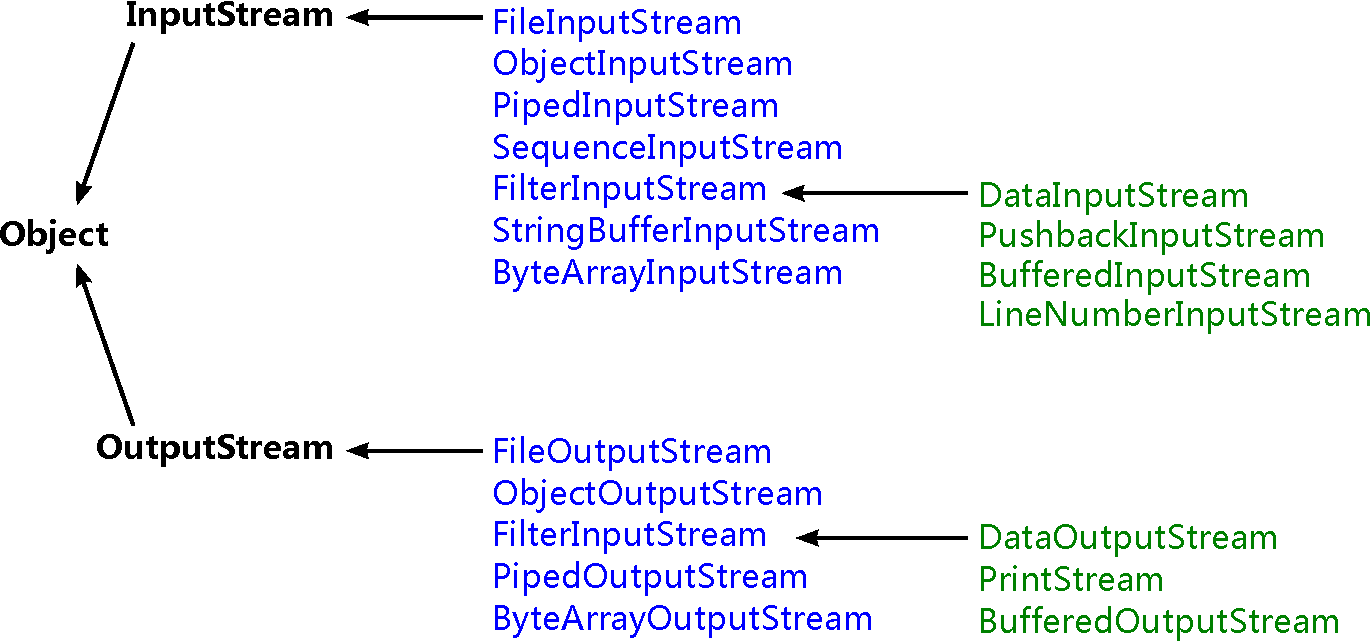
\includegraphics[width=0.8\textwidth]{images/Advanced-IO-programming/fig-io-input-and-output-stream.pdf}
\caption{InputStream和OutputStream}
\label{fig:fig-io-input-and-output-stream}
\end{figure}

\subsection{InputStream}

抽象类java.io.InputStream是所有字节输入流类型的父类,该类中定义了以字节为单
位读取数据的基本方法,并在其子类中进行了分化和实现。

\subsubsection{三个基本的read方法}

\begin{itemize}
\item int read()
\item int read(byte[] buffer)
\item int read(byte[] buffer, int offset, int length)
\end{itemize}

\subsubsection{其它方法}

\begin{itemize}
\item void close()
\item int available()
\item skip(long n)
\item boolean markSupported()
\end{itemize}

\subsection{OutputStream}

java.io.OutputStream与java.io.InputStream对应,是所有字节输出流类型的抽象父类。

\subsubsection{三个基本的write方法}

\begin{itemize}
\item void write(int c)
\item void write(byte[] buffer)
\item void write(byte[] buffer, int offset, int length)
\end{itemize}

\subsubsection{其它方法}

\begin{itemize}
\item void close()
\item void flush()
\end{itemize}

\subsection{Reader and Writer}

\begin{figure}[htb]
\centering
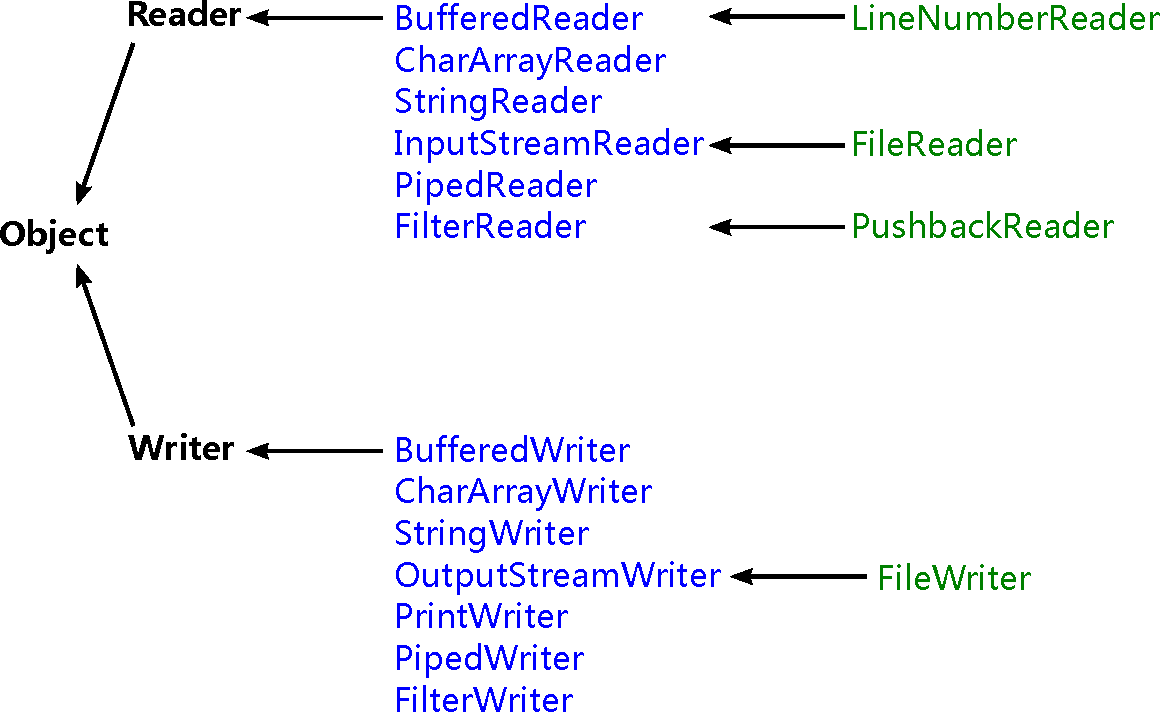
\includegraphics[width=0.8\textwidth]{images/Advanced-IO-programming/fig-io-reader-and-writer.pdf}
\caption{InputStream和OutputStream}
\label{fig:fig-io-reader-and-writer}
\end{figure}

\subsection{Reader}

抽象类java.io.Reader是所有字符输入流类型的父类,其中声明了用于读取字符流的有关方法。

\subsubsection{三个基本的read方法}

\begin{itemize}
\item int read()
\item int read(char[] cbuf)
\item int read(char[] cbuf, int offset, int length)
\end{itemize}

\subsubsection{其它方法}

\begin{itemize}
\item void close()
\item boolean ready()
\item skip(long n)
\item boolean markSupported()
\item void mark(int readAheadLimit)
\end{itemize}

\subsection{Writer}

java.io.Writer与java.io.Reader类对应,是所有字符输出流类型的共同父类。

\subsubsection{五个基本的write方法}

\begin{itemize}
\item void write(int c)
\item void write(char[] cbuf)
\item void write(char[] cbuf, int offset, int length)
\item void write(String string)
\item void write(String string, int offset, int length)
\end{itemize}

\subsubsection{其它方法}

\begin{itemize}
\item void close()
\end{itemize}

\section{常用I/O流类型}

\subsection{FileInputStream/FileOutputStream}

\begin{itemize}
\item FileInputStream用于读取本地文件中字节数据,FileOutputStream用于将
  字节数据写出到文件。
\item FilenputStream不适合获取文本文件中的字符信息,要读取并显示的文件
  中如果含有双字节字符(如中文),则会显示乱码,此时应该采用字符流类
  型。
\item {\Red \it 可以用于复制任何格式的文件,如文本、音视频以及可执行文
    件等二进制文件,因为以字节为单位进行数据复制时并不对文件内容进行解
    析。}
\end{itemize}

\samp{Fragment: 使用字节流实现文件复制}

\begin{javaCode}
  FileInputStream fis = new FileInputStream("in.txt");
  FileOutputStream fos = new FileOutputStream("out.txt");
  int read = fis.read();
  while (read != -1) {
    fos.write(read);
    read = fis.read();
  } 
  fis.close();
  fos.close();
\end{javaCode}

\subsection{FileReader/FileWriter}

\begin{itemize}
\item FileReader用于以{\hei 字符}为单位读取文本文件,FileWriter类用于将字符数据写出到文
  本文件。
\item 字符I/O流类型只能处理文本文件,因为二进制文件中保存的字节信息不能正常解析为字符。
\end{itemize}

\samp{Fragment: 使用字符流实现文件复制}

\begin{javaCode}
  FileReader fis = new FileReader("in.txt");
  // The second arg is boolean append, true for appending, false for covering.
  FileWriter fos = new FileWriter("out.txt", true); 
  int read = fis.read();
  while (read != -1) {
    fos.write(read);
    read = fis.read();
  } 
  fis.close();
  fos.close();
\end{javaCode}

\subsection{BufferedReader/BufferedWriter}

\begin{itemize}
\item BufferedReader用于缓冲读取字符、字符数组或行,采用缓冲处理能够提高效率,该类所封装
  的字节输入流对象需要在构造方法中指定。
  
  \begin{itemize}
  \item public BufferedReader(Reader in)
  \item public BufferedReader(Reader in, int size) // size of buffer
  \end{itemize}
\item BufferedWriter提供字符的缓冲写出功能,该类的newLine()方法可以写出平台相关的行分隔符
  来标记一行的终止,此分割符由系统属性line.separator确定。
\end{itemize}

\samp{Fragment: 使用字符处理流实现文件复制}

\begin{javaCode}
  BufferedReader br = new BufferedReader(new FileReader("in.txt"));
  BufferedWriter bw = new BufferedWriter(new FileWriter("out.txt"));
  String s = br.readLine();
  while (s != null) {
    bw.write(s);
    bw.newLine(); // notice.
    s = br.readLine();
  }
\end{javaCode}

\subsection{Other I/O Classes}
\begin{itemize}
\item InputStreamReader/OutputStreamWriter
\item PrintStream/PrintWriter
\item DataInputStream/DataOutputStream
\item CharArrayReader/CharArrayWriter
\end{itemize}

\section{I/O应用}

\subsection{属性信息的导入/导出}

如果要永久记录用户自定义的属性,可以采用Properties类的load()/store()方
法进行属性的导入/导出操作,即将属性信息写出到文件中和从文件中读取属性信
息到程序。

\samp{SaveProperties.java}

\begin{javaCode}
  import java.io.FileWriter;
  import java.util.Properties;
  public class SaveProperties {
    public static void main(String[] args) {
      try {
        Properties ps = new Properties();
        ps.setProperty("name", "Kevin");
        ps.setProperty("password", "12345");
        FileWriter fw = new FileWriter("props.txt");
        ps.store(fw, "loginfo");
        fw.close();
      } catch (Exception e) {
        e.printStackTrace();
      }
    }
  }
\end{javaCode}

\subsection{属性信息的导入/导出}

\samp{LoadProperties.java}

\begin{javaCode}
  import java.io.FileWriter;
  import java.util.Properties;
  public class LoadProperties {
    public static void main(String[] args) {
      try {
        Properties ps = new Properties();
        FileReader fr = new FileReader("props.txt");
        ps.load(fr);
        fr.close();
        ps.list(System.out);
      } catch (Exception e) {
        e.printStackTrace();
      }
    }
  }
\end{javaCode}

文件props.txt内容如下:

\begin{shCode}
#loginfo
#Sun Nov 04 21:20:17 CST 2012
password=12345
name=Kevin
\end{shCode}

标准输出如下:

\begin{stdoutCode}
-- listing properties --
password=12345
name=Kevin
\end{stdoutCode}

\subsection{对象序列化}

\subsubsection{概念}

对象序列化(Object Serialization)是指将对象的状态数据以字节流的形式进
行处理,一般用于实现对象的持久性,即长久保存一个对象的状态并在需要时获
取该对象的信息以重新构造一个状态完全相同的对象。对象序列化可以理解为使
用I/O“对象流”类型实现对象读/写操作。

\begin{itemize}\kai
\item {\hei 对象的持久性(Object Persistance)} 长久保存一个对象的状态
  并在需要时获取该对象的信息以重新构造一个状态完全相同的对象。
\item {\hei 对象序列化(Object Serialization)} 通过写出对象的状态数据
  来记录一个对象。
\item {\hei 对象序列化的主要任务} 写出对象的状态信息,并遍历该对象对其
  他对象的引用,递归的序列化所有被引用到的其他对象,从而建立一个完整的
  序列化流。
\end{itemize}

\subsection{实现对象序列化}

要序列化一个对象,其所属的类必须实现以下两种接口之一:

\begin{itemize}
\item java.io.Serializable
\item java.io.Externalizable
\end{itemize}

java.io.ObjectOutputStream和ObjectInputStream类分别提供了对象的序列化和反序列化功能。

\notice{注意}

\begin{itemize}\kai
\item 在对象序列化过程中,其所属类的static属性和方法代码不会被序列化;
\item 对于个别不希望被序列化的非static属性,也可以在属性声明的时候使用transient关键字进行标明。
\end{itemize}

\codeset{sample.io.serialization}


%%%%\begin{frame}[fragile] % [fragile]参数使得能够插入代码
%%%%\subsection{标准输入输出重定向}
%%%%
%%%%Java控制台程序默认是以控制台键盘和显示器作为标准输入/输出设备,在有些有情况下,我们可能希望将程序的标准输入或标准输出进行重新定向。
%%%%
%%%%{\kai\Blue 例如,程序测试时可能需要大量数据,如果使用控制台输入测试数据的话每次都要重新输入,这样很繁琐,此时可以考虑进行输入重定向。}
%%%%\end{frame}
%%%%
%%%%\begin{frame}[fragile] % [fragile]参数使得能够插入代码
%%%%  \subsection{标准输入输出重定向}
%%%%  
%%%%  \samp{TestSetInput.java}
%%%%  \begin{javaCode}
%%%%    import java.io.*;
%%%%    public class TestSetInput {
%%%%      public static void main(String[] args) {
%%%%        try {
%%%%          FileInputStream fis = new FileInputStream("in.txt");
%%%%          System.setIn(fis);
%%%%          int avg = 0;
%%%%          int total = 0;
%%%%          int num = 0;
%%%%          int i;
%%%%          BufferedReader br = new BufferedReader(new InputStreamReader(System.in));
%%%%          String s = br.readLine();
%%%%          while (s != null && !s.equals("over")) {
%%%%            i = Integer.parseInt(s);
%%%%            num++;
%%%%            total += i;
%%%%            avg = total / num;
%%%%            System.out.println("num=" + num + "\ttotal=" + total + "\tavg=" + avg);
%%%%            s = br.readLine();
%%%%          }
%%%%        } catch (IOException e) {
%%%%          e.printStackTrace();
%%%%        }
%%%%      }
%%%%    }
%%%%\end{javaCode}
%%%%其中,in.txt为每行均为整数的文件。
%%%%\end{frame}
%%%%
%%%%\begin{frame}[fragile] % [fragile]参数使得能够插入代码
%%%%\subsection{标准输入输出重定向}
%%%%\begin{itemize}
%%%%\item System.setOut(OutputStream output)
%%%%\item System.setErr(OutputStream output)
%%%%\end{itemize}
%%%%\end{frame}
%%%%
%%%%\begin{frame}[fragile] % [fragile]参数使得能够插入代码
%%%%\subsection{随机存取文件}
%%%%\tta{需求}
%%%%\begin{itemize}
%%%%\item 存档游戏,记录新玩家的第一次成绩时,添加一条新纪录。
%%%%\item 老用户重玩时,更新其原有记录信息(不添加新纪录)。
%%%%\item 浏览所有玩家的记录信息。
%%%%\end{itemize}
%%%%
%%%%\tta{一种实现方式} \\
%%%%使用java.io.RandomAccessFile类实现文件的随机存取操作,该方法能够同时提
%%%%供读/写文件的功能。\footnote{代码见tex源文件 :)}
%%%%
%%%%%%%%%%%%%%%%%%%%%%%%%%%%%%%%%%%%%%%%%%%%%%%%%%%%%%%%%%%%%%%%%%%%%%
%%%%% \begin{javaCode}
%%%%% import java.io.File;
%%%%% import java.io.IOException;
%%%%% import java.io.RandomAccessFile;
%%%%% public class TestRandomAccessFile {
%%%%%   private File file = null;
%%%%%   public void record(String record_breaker, int times) {
%%%%%     try {
%%%%%       RandomAccessFile raf = new RandomAccessFile(file, "rw");
%%%%%       boolean flag = false;
%%%%%       while (raf.getFilePointer() < raf.length()) {
%%%%%         String name = raf.readUTF();
%%%%%         if (record_breaker.equals(name)) {
%%%%%           raf.writeInt(times);
%%%%%           flag = true;
%%%%%           break;
%%%%%         } else {
%%%%%           raf.skipBytes(4);
%%%%%         }
%%%%%       }
%%%%%       if (!flag) {
%%%%%         raf.writeUTF(record_breaker);
%%%%%         raf.writeInt(times);
%%%%%       }
%%%%%       raf.close();
%%%%%     } catch (Exception e) {
%%%%%       e.printStackTrace();
%%%%%     }
%%%%%   }
%%%%%   public void init() {
%%%%%     if (file == null) {
%%%%%       file = new File("record.txt");
%%%%%       try {
%%%%%         file.createNewFile();
%%%%%       } catch (IOException e) {
%%%%%         e.printStackTrace();
%%%%%       }
%%%%%     }
%%%%%   }
%%%%%   public void listAllRecords() {
%%%%%     try {
%%%%%       RandomAccessFile raf = new RandomAccessFile(file, "r");
%%%%%       while (raf.getFilePointer() < raf.length()) {
%%%%%         String name = raf.readUTF();
%%%%%         int times = raf.readInt();
%%%%%         System.out.println("name: " + name + "\trecord: " + times);
%%%%%       }
%%%%%       raf.close();
%%%%%     } catch (Exception e) {
%%%%%       e.printStackTrace();
%%%%%     }
%%%%%   }
%%%%%   public static void main(String[] args) {
%%%%%     TestRandomAccessFile traf = new TestRandomAccessFile();
%%%%%     traf.init();
%%%%%     traf.record("Billy", 30);
%%%%%     traf.record("Kevin", 32);
%%%%%     traf.listAllRecords();
%%%%%   }
%%%%% }
%%%%% \end{javaCode}
%%%%%%%%%%%%%%%%%%%%%%%%%%%%%%%%%%%%%%%%%%%%%%%%%%%%%%%%%%%%%%%%%%%%%%
%%%%\end{frame}


\section{课后习题}

\tta{简答题}

\begin{enumerate}
\item 概述Java I/O流的分类。
\item 总结补全幻灯片中基础I/O流部分各方法的功能和用法。
\end{enumerate}

\tta{小编程}

\begin{enumerate}
\item 编程实践任意类型文件和文本文件复制代码。
\item 编程实践属性信息的导入导出代码。
\item 编程实践对象序列化代码。
\end{enumerate}